% Options for packages loaded elsewhere
\PassOptionsToPackage{unicode}{hyperref}
\PassOptionsToPackage{hyphens}{url}
\documentclass[
  ignorenonframetext,
]{beamer}
\newif\ifbibliography
\usepackage{pgfpages}
\setbeamertemplate{caption}[numbered]
\setbeamertemplate{caption label separator}{: }
\setbeamercolor{caption name}{fg=normal text.fg}
\beamertemplatenavigationsymbolsempty
% remove section numbering
\setbeamertemplate{part page}{
  \centering
  \begin{beamercolorbox}[sep=16pt,center]{part title}
    \usebeamerfont{part title}\insertpart\par
  \end{beamercolorbox}
}
\setbeamertemplate{section page}{
  \centering
  \begin{beamercolorbox}[sep=12pt,center]{section title}
    \usebeamerfont{section title}\insertsection\par
  \end{beamercolorbox}
}
\setbeamertemplate{subsection page}{
  \centering
  \begin{beamercolorbox}[sep=8pt,center]{subsection title}
    \usebeamerfont{subsection title}\insertsubsection\par
  \end{beamercolorbox}
}
% Prevent slide breaks in the middle of a paragraph
\widowpenalties 1 10000
\raggedbottom
\AtBeginPart{
  \frame{\partpage}
}
\AtBeginSection{
  \ifbibliography
  \else
    \frame{\sectionpage}
  \fi
}
\AtBeginSubsection{
  \frame{\subsectionpage}
}
\usepackage{iftex}
\ifPDFTeX
  \usepackage[T1]{fontenc}
  \usepackage[utf8]{inputenc}
  \usepackage{textcomp} % provide euro and other symbols
\else % if luatex or xetex
  \usepackage{unicode-math} % this also loads fontspec
  \defaultfontfeatures{Scale=MatchLowercase}
  \defaultfontfeatures[\rmfamily]{Ligatures=TeX,Scale=1}
\fi
\usepackage{lmodern}
\ifPDFTeX\else
  % xetex/luatex font selection
\fi
% Use upquote if available, for straight quotes in verbatim environments
\IfFileExists{upquote.sty}{\usepackage{upquote}}{}
\IfFileExists{microtype.sty}{% use microtype if available
  \usepackage[]{microtype}
  \UseMicrotypeSet[protrusion]{basicmath} % disable protrusion for tt fonts
}{}
\makeatletter
\@ifundefined{KOMAClassName}{% if non-KOMA class
  \IfFileExists{parskip.sty}{%
    \usepackage{parskip}
  }{% else
    \setlength{\parindent}{0pt}
    \setlength{\parskip}{6pt plus 2pt minus 1pt}}
}{% if KOMA class
  \KOMAoptions{parskip=half}}
\makeatother
\usepackage{graphicx}
\makeatletter
\newsavebox\pandoc@box
\newcommand*\pandocbounded[1]{% scales image to fit in text height/width
  \sbox\pandoc@box{#1}%
  \Gscale@div\@tempa{\textheight}{\dimexpr\ht\pandoc@box+\dp\pandoc@box\relax}%
  \Gscale@div\@tempb{\linewidth}{\wd\pandoc@box}%
  \ifdim\@tempb\p@<\@tempa\p@\let\@tempa\@tempb\fi% select the smaller of both
  \ifdim\@tempa\p@<\p@\scalebox{\@tempa}{\usebox\pandoc@box}%
  \else\usebox{\pandoc@box}%
  \fi%
}
% Set default figure placement to htbp
\def\fps@figure{htbp}
\makeatother
\setlength{\emergencystretch}{3em} % prevent overfull lines
\providecommand{\tightlist}{%
  \setlength{\itemsep}{0pt}\setlength{\parskip}{0pt}}
% Slide layout defaults for warning-clean scientific decks.
\usepackage{etoolbox}
\IfFileExists{xurl.sty}{\usepackage{xurl}}{}
\IfFileExists{seqsplit.sty}{\usepackage{seqsplit}}{\newcommand{\seqsplit}[1]{#1}}
\protected\def\breakseq#1{\seqsplit{#1}}
\protected\def\breaktt#1{\begingroup\ttfamily\seqsplit{#1}\endgroup}
\setlength{\emergencystretch}{6em}
\tolerance=5000
\hbadness=10000
\hfuzz=1pt
\setlength{\tabcolsep}{2pt}
\AtBeginEnvironment{longtable}{\tiny\renewcommand{\arraystretch}{0.86}\setlength{\tabcolsep}{1pt}}
\AtBeginEnvironment{tabular}{\tiny\renewcommand{\arraystretch}{0.86}\setlength{\tabcolsep}{1pt}}

% Natbib and cross-reference fallbacks — slides don't load natbib
% or cleveref, but combined-PDF manuscript prose may emit these
% commands. The fallback renders citations as a bracketed key list
% and cross-references as detokenized labels so slides don't fail on
% undefined control sequences or raw underscores. \providecommand is
% a no-op if packages load later.
\providecommand{\citep}[1]{[#1]}
\providecommand{\citet}[1]{#1}
\providecommand{\citealp}[1]{#1}
\providecommand{\citeauthor}[1]{#1}
\providecommand{\citeyear}[1]{#1}
\providecommand{\cref}[1]{\texttt{\detokenize{#1}}}
\providecommand{\Cref}[1]{\texttt{\detokenize{#1}}}

\newtheorem{proposition}{Proposition}
\newtheorem{hypothesis}{Hypothesis}
\usepackage{bookmark}
\IfFileExists{xurl.sty}{\usepackage{xurl}}{} % add URL line breaks if available
\urlstyle{same}
% fallback for those not using the hyperref driver hyperxmp:
\makeatletter
\@ifundefined{xmpquote}{\newcommand{\xmpquote}[1]{#1}}{}
\makeatother
\hypersetup{
  hidelinks,
  pdfcreator={LaTeX via pandoc}}

\author{\texorpdfstring{}{}}
\date{}

\begin{document}

\section{Place-Based Micropractice and Digital
Placemaking}\label{sec:place}

\begin{frame}[fragile,allowframebreaks]{Place-Based Micropractice and
Digital Placemaking}
Place-based DigiPPPiP treats the drawing context as part of the
relational artifact. A shared canvas can carry marks from a kitchen
table, a hospital room, a train, a park, or two distant cities. CSCW
place theory distinguishes lived place from abstract space, which
matters because a canvas becomes place-like only through situated
practice and shared interpretation \breakseq{[@dourish2006respace]}.
Place-attachment research and networked-locality and digital-placemaking
scholarship show that digital media can intensify rather than dissolve
place attachment when it is designed to connect people, memory, and
environment \breakseq{[@lewicka2011place; @gordon2011netlocality;
@foth2015digitalcity; @canelas2025placemaking]}. The relevant unit is
small: a canvas can become a relational micro-place even if it never
becomes a public platform or civic interface.

Place-responsive DigiPPPiP asks each partner to draw from their
immediate environment. One partner may contribute a window view; another
may respond with a local sound, map trace, color palette, or remembered
path. The result is neither a private diary nor a generic online
whiteboard. It is a relational place object: two embodied situations
negotiated on one shared surface. Place claims should remain qualitative
until participants describe particular canvases as meaningful places.

The minimum place claim requires recurrence, situated reference, and
shared uptake. A one-time location tag is only metadata; a repeated
drawing practice can become place-responsive when partners return to
recognizable cues and use them to coordinate memory, mood, or care. This
boundary keeps placemaking from becoming a decorative label for any
geolocated canvas.

A place-responsive protocol should therefore ask what place cue is being
shared, who chose it, how precise it needs to be, and whether either
partner wants it excluded from storage or export. The cue can be coarse:
room type, local weather, a remembered path, an object on the table, a
hospital routine, or a neighborhood sound. Precise global positioning
system (GPS) coordinates are not required for the framework claim and
may be inappropriate when the canvas is intimate, health-adjacent, or
used by a vulnerable participant. The research record should preserve
the prompt category and consent state without turning place into
surveillance.

\breakseq{[@fig:relational\_microplaces]} maps this scale. The figure treats
kitchens, studios, hospital rooms, trains, and two-city routines as
contexts that can feed a persistent canvas. The point is not that a
digital artifact automatically creates place attachment; it is that
repeated return, situated prompts, and shared memory can make a canvas
function like a small relational place.

\begin{figure}
\centering
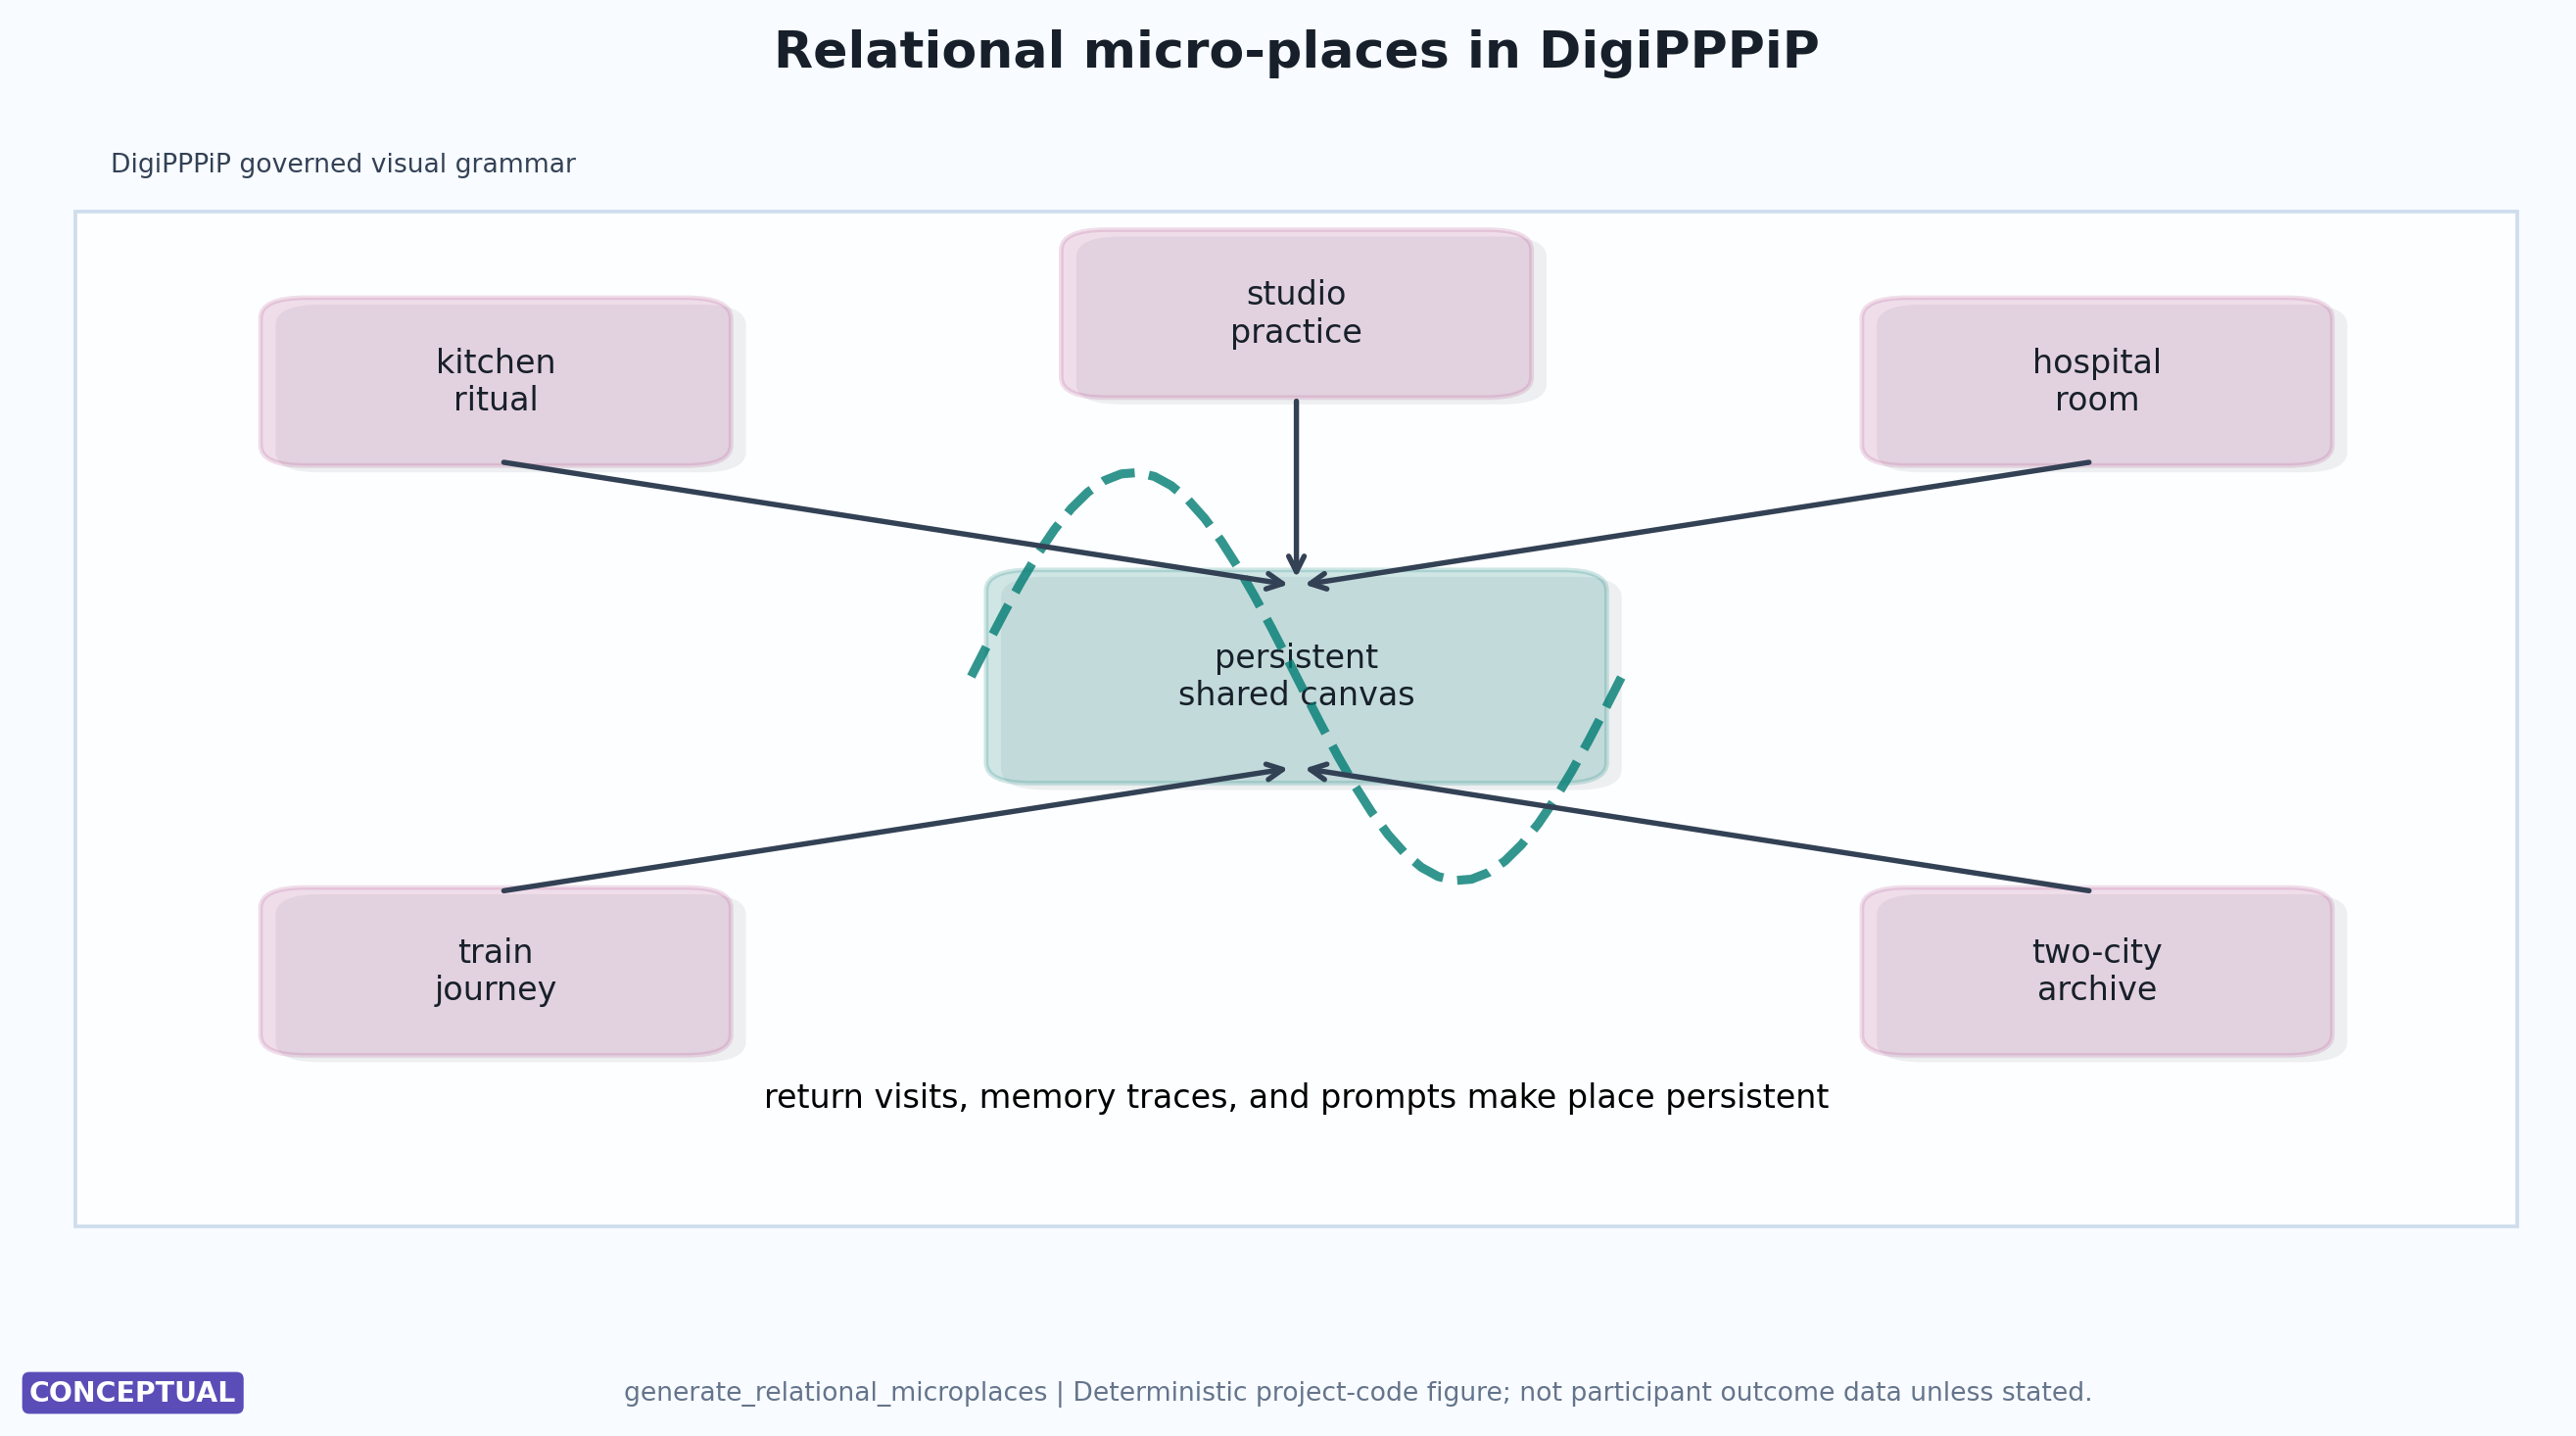
\includegraphics[width=0.9\linewidth,height=0.46\textheight,keepaspectratio,alt={Digital placemaking map for recurring DigiPPPiP relational micro-places. The figure is generated by generate\_relational\_microplaces(); read the peripheral place boxes as situated contexts and the central artifact as a persistent canvas that can be revisited. It supports the place-based claim that recurrence and shared uptake matter more than geolocation alone. The diagram is conceptual and does not imply surveillance, community-scale impact, or universal place attachment.}]{../figures/relational_microplaces.png}
\caption{Digital placemaking map for recurring DigiPPPiP relational
micro-places. The figure is generated by
\protect\breaktt{generate\_relational\_microplaces()}; read the
peripheral place boxes as situated contexts and the central artifact as
a persistent canvas that can be revisited. It supports the place-based
claim that recurrence and shared uptake matter more than geolocation
alone. The diagram is conceptual and does not imply surveillance,
community-scale impact, or universal place
attachment.}\label{fig:relational_microplaces}
\end{figure}

This place dimension is especially useful for long-distance partners and
communities. A remote digital mode can support geographic reach, but
place-responsive prompts keep the practice situated. The taxonomy in
\breakseq{[@fig:taxonomy\_matrix]} captures this as a trade-off between
geographic reach and place grounding rather than a binary opposition
between online and offline.
\end{frame}

\end{document}
